\section{Majorana fermions and topological superconductors}

We discuss here MFs, their connection to topological superconductors, and the properties that can be exploited for topological quantum computing.
%Before we define Majorana fermions we will discuss characteristics of fermions.
Fermions are particles that follow Fermi-Dirac statistics and the Pauli exclusion principle and have half-integer spin (spin 1/2, 3/2, etc.). There are three types of fermions: Dirac, Weyl, and Majorana. 
In 1926, both Enrico Fermi and Paul Dirac derived Fermi-Dirac statistics independently.
Dirac's equation led to the derivation of a (complex) wavefunction solution for spin-half fermions that have mass and charge, and an antiparticle, coined as the positron.
A few years later, Hermann Weyl derived from Dirac's equation a simplified solution for describing massless fermions.
Then, in 1937 Ettore Majorana hypothesized from Dirac's equation a (real) wavefunction solution that showed that these fermions were their own antiparticles and neutrally charged.

Examples of observed fermions include electrons, neutrinos, neutrons, and protons.
%Weyl and Majorana fermions have yet to be observed.
The Standard Model does allow for neutrinos to potentially be MFs.
The MAJORANA project: neutrinoless double beta decay, is one experiment for detecing neutrino MFs and has yielded negative results thus far.
The particle physics community has yet to find either Weyl or MFs in experiments.
There are, however, avenues for pursuing them as quasiparticles in condensed matter systems.
For example, in 2011 Weyl fermions were theorized to be in topological semimetals then quickly observed as quasiparticles by 2015 in TaAs semimetals using angle-resolved photoemission spectroscopy (ARPES)  ~\cite{wanTopologicalSemimetalFermiarc2011, xuDiscoveryWeylFermion2015, liWeylSemimetalTaAs2016}.
Since 2001 it has been hypothesized that MFs can be found in \textit{p}-wave superconductors in pairs, either at cores of half-quantum vortices or at the ends of wires.

In conventional superconductors there are Cooper pairs that support supercurrents.
These Cooper pairs are made up of two electrons (or holes) with opposite spin and momenta caused by the electron-phonon interaction.
A Bogoliubov quasiparticle is the first excited state of a Cooper pair condensate.
This is when an electron and hole with opposite momenta become paired.
Tuning the system's chemical potential allows the electron and hole bands to cross one another in the Brillouin zone.
The superconducting order parameter, $\Delta$, dictates the type of spinful coupling for the Bogoliubov quasiparticles.
For example, superconductors that are \textit{s}-wave, pair electrons and holes with opposite spin, while \textit{p}-wave ones pair electrons and holes that compose spin-triplets.
In a \textit{p}-wave superconductor, if the Bogoliubov quasiparticle is a zero-energy excitation, it can be written as a highly non-local Majorana zero mode (MZM).
MZMs come in pairs due to particle-hole symmetry of the system.

There are a few reasons why MFs are highly sought after:
MFs are dictated by non-Abelian exchange statistics, which allows for building a universal quantum computer.
Another perk of non-trivial topological superconductors, is the ability to protect MFs from local perturbations, also known as fault-tolerant.
This reduces the error that qubits can acquire when performing a braiding operation.
The next few subsections will review these properties of MFs in topological superconductors.

\subsection{Kitaev chain}
We now review the Kitaev chain, a realization of MZMs, or MFs, on a 1D spinless \textit{p}-wave superconductor.
The derivation can be found in the following reference ~\cite{kitaevUnpairedMajoranaFermions2001}.
Originally, Kitaev's proposal was to design a topological quantum storage device.
However, a Kitaev chain can be used for more than storage: it is a key building block in constructing topological quantum logic gates.

Start with a 1D spinless \textit{p}-wave superconductor tight-binding Hamiltonian

\begin{equation}
  \ham = \sum_j^{N-1} (-t \cc_j c_{j+1} + \Delta c_j c_{j+1} + h.c.) - \sum_j^{N} \mu \cc_j c_j,
\end{equation}
where $t$ is hopping amplitude, $\Delta = |\Delta|$ is the superconducting order parameter, $\mu$ is chemical potential, and $\cc (c)$ is the creation (annihilation) operator for a complex fermion.
We use the following MF basis transformation: $\cc_j = \tfrac{1}{2} (a_j - i b_j)$, where $\left\{ a^{\dagger}_j, a_{j'} \right\} = \left\{ a_j, a_{j'} \right\} = 2\delta_{j,j'}$ and $\left\{a_j,b_{j'}\right\} = 0$.
The Hamiltonian becomes

\begin{equation}
  \ham = \dfrac{i}{2} \sum_j \left( -\mu a_j b_j + (t+\Delta) b_j a_{j+1} + (-t+\Delta) a_j b_{j+1} \right).
\end{equation}
A trivial topology phase, meaning there are no MFs at chain ends, can be achieved by having $\mu \neq 0$ and $t=\Delta=0$, leading to

\begin{equation}
  \ham = -\mu\dfrac{1}{2} \sum_j a_j b_j.
\end{equation}
The non-trivial topology phase, in which there are MFs present at chain ends, can be realized by setting $\mu = 0$, and $t = \Delta > 0$:

\begin{equation}
  \ham = it \sum_j b_j a_{j+1}.
\end{equation}
Notice terms $a_1$ and $b_N$ are missing in the non-trivial topology Hamiltonian.
We define the non-localized zero energy mode present in the system as the following fermionic operator, $f = \tfrac{1}{2}(a_1 + i b_N)$.
This state is composed of two well separated MZMs.
Figure ~\ref{fig:kitaev-chain} shows the wire in both topological phases.

\begin{figure}
  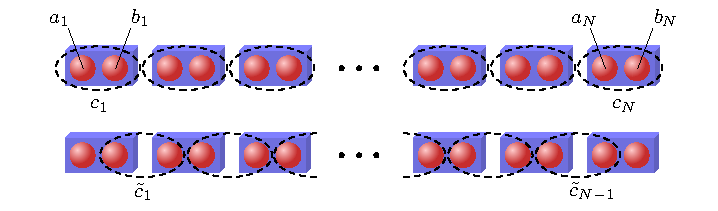
\includegraphics[width=\textwidth]{./figures/kitaev-chain.pdf}
  \caption{The top chain represents the system in a trivial topology where each complex fermion $c_j = \tfrac{1}{2}(a_j + i b_j)$ is a linear combination of intraconnected MFs. The bottom chain represents the system in a non-trivial topology where each complex fermion $\tilde{c}_j = \tfrac{1}{2}(a_j + i b_{j+1})$ is a linear combination of interconnected MFs, leaving the non-localized complex fermion $f = \tfrac{1}{2}(a_1 + i b_N)$, and thus leaving one MF located at each end of the chain.}
  \label{fig:kitaev-chain}
\end{figure}

Slightly outside the Kitaev limit, a non-trivial topology persists if $|\mu| < 2t$ and $t = |\Delta| >0$.
Due to bulk-edge correspondence, MZMs are localized at the interface between trivial and non-trivial segments.
To formalize this, we calculate the topological invariant, known as the Majorana number.
While calculating the Majorana number is straightforward enough, its proof, shown in  App. \ref{app:majorana-number}, is not.
To compute the Majorana number, we perform a MF basis transformation on the Hamiltonian, $A = -iU \ham U^{\dagger}$, then take the sign of the Pfaffian,

\begin{equation}
  \mathcal{M} = \text{sgn} [\text{Pf} (A)].
\end{equation}
If the system has translational symmetry in the chain direction, the Hamiltonian can be transformed into momentum space.
Using the symmetry condition $\epsilon(-k) = -\epsilon(k)$, we find that for any given $k$, there are equal numbers of positive and negative eigenvalues.
The Majorana number then simplifies to

\begin{equation}
  \mathcal{M} =
  \begin{cases}
    \text{sgn} [\text{Pf} (A_{k=0}) \text{Pf} (A_{k=\pi})], &\text{if L is even}, \\
    \text{sgn} [\text{Pf} (A_{k=0})], &\text{if L is odd},
  \end{cases}
\end{equation}
where L is the number of lattice sites.
Within the Kitaev limit, if $|\mu|< 2t$, then $\mathcal{M} = -1$, and if $|\mu| > 2t$, then $\mathcal{M} = 1$.
If one section of the material exhibits non-trivial topology while adjacent sections remain trivial, MZMs will localize at interfaces of differing topological numbers.
This phenomena is a direct consequence of bulk-edge correspondence.

Now that we have a way to distinguish topological states, we must consider the size of the systems band gap and robustness.
When $|\mu| = 2t$, the system reaches a critical point where the band gap opens and closes, making this region of parameter space undesirable.
A too small band gap allows even minor local perturbations to reopen or close it and therefore compromises the stability and information of the MZMs.
By tuning the chemical potential further from these critical points, the band gap becomes larger, increasing robustness against local perturbations.


But what are local perturbations and how do they contribute to error?
There are two common types of error in quantum computers: classical and phase.
Classical error flips the qubit state, $|1\rangle \rightarrow |0\rangle$ and vice versa.
Phase error changes the sign of the occupied state, $|1\rangle \rightarrow -|1\rangle$, relative to the unoccupied state $|0\rangle$. To get rid of the classical error we can envision the following: Imagine an electron hopping from one site to another, creating two classical errors simultaneously.
If our fermionic qubit state has its information distributed non-locally in MZMs, the possibility of an electron hopping between the two MZMs becomes exponentially small with separation distance.
Simply put, the error must affect both MZMs at the same time which is highly unlikely given a large separation.

Phase error can be represented as $\cc_j c_j$, leading to different electron configurations acquiring different phases over time.
Majorana operators as defined earlier give the following phase error operator $\cc_j c_j = \frac{1}{2} (1+ i a_j b_j)$.
This would require the highly non-local MZMs to share the same site to induce a phase error.
In summary, non-trivial topology makes MZMs difficult to couple together due to their separation and a large band gap prevents excitations.
~\cite{kitaevUnpairedMajoranaFermions2001}.


\subsection{Half-quantum vortices in \textit{p}-wave superconductors}
We now transition to Ivanov's derivation of MFs \cite{ivanovNonAbelianStatisticsHalfQuantum2001} and introduce \textit{braiding} for their topological quantum computing applications.
It was proposed by Read and Green that the Pfaffian quantum Hall state derived by Moore and Read belongs to the same topological class as the Bardeen-Cooper-Schrieffer (BCS) pairing state.
Ivanov later verified that this was the case: BCS states in $p$-wave superconductors exhibit non-Abelian statistics in the presence of half-quantum vortices.
To explicitly show this, we first need to understand how the superconducting order parameter acts under different pairing potentials composed of singlet or triplet states.

The superconducting order parameter, also called order parameter or pairing potential for short, tells us the correlation between two fermionic operators in a superconductor and requires the state to be antisymmetric.
The order parameter is made up of a spatial and spin component, with symmetry constraints dictating their relationship.
In spin-singlet pairing, the spin component is antisymmetric, limiting the spatial component to be symmetric.
This occurs in \textit{s}- and \textit{d}-wave superconductors.
In spin-triplet pairing, the spin component is symmetric, limiting the spatial component to be antisymmetric.
This occurs in \textit{p}- and \textit{f}-wave superconductors.

In terms of Pauli matrices, the order parameter can be expressed as

\begin{equation}
  \Delta (\vec{k}) = \left(\Delta_0 (\vec{k}) + \vec{d}(\vec{k}) \cdot \bm{\sigma}\right) i \sigma_y,
\end{equation}
where the antisymmetric condition $\Delta(\vec{k}) = \Delta^T(-\vec{k})$ encodes $\Delta_0 (\vec{k})$ as spin-singlet components and $\vec{d}(\vec{k})$ as spin-triplet components, and $\sigma_y$ maintains the overall antisymmetric nature of the matrix.
The direction vector $\vec{d}$ must be a three dimensional vector to ensure the three spin configurations
$|\uparrow\uparrow\rangle$, $|\uparrow\downarrow\rangle + |\downarrow\uparrow\rangle$, and $|\downarrow\downarrow\rangle$.
The parity of the spatial component determines $\Delta(\vec{k})$.
Even-parity is of even powers in momentum, proportional to even spherical harmonics.
Odd-parity is of odd powers in momentum, proportional to odd spherical harmonics.
For example, in \textit{s}-wave superconductors $l=0$, the spherical harmonic $Y_{0,0}$ is constant and has no momentum dependence and takes the form
$\Delta_s (\vec{k}) = i\Delta_0 \sigma_y$.
In contrast, for \textit{p}-wave superconductors $l=1$, the spherical harmonic $Y_{1,\pm1} \propto k_x \pm i k_y$, leading to linear dependence in momentum.
This leads to the order parameter
$\Delta_p(\vec{k}) = i\Delta (\vec{d} \cdot \bm{\sigma}) (k_x+ik_y) \sigma_y$.
In a word, the symmetry of the superconducting state determines the structure of $\Delta(\vec{k})$ and how it influences the physical properties of the system.

\begin{figure}
  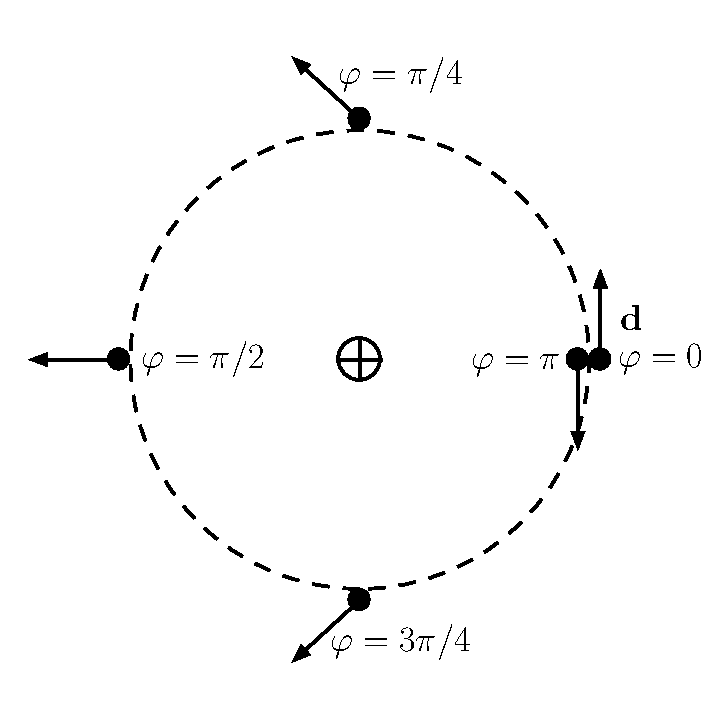
\includegraphics[width=0.4\textwidth]{./figures/half-quantum-vortex.pdf}
  \caption{The order phase $\varphi$ and angle $\alpha$ of $\vec{d}$ rotate by $\pi$: ($\varphi , \vec{d}$) \rightarrow ($\varphi+\pi, -\vec{d}$). The order parameter $\theta$ maps to itself, ($0, 2\pi$), under simultaneous change of both $\vec{d}$ and $\varphi$: $\theta = \varphi + \alpha$.}
  \label{fig:half-quantum-vortex}
\end{figure}

In Ivanov's proof \cite{ivanovNonAbelianStatisticsHalfQuantum2001}, a slightly different basis for the triplet-pairing order parameter is used

\begin{equation}
  %\Delta (\vec{k}) = \Delta e^{i\phi} \left[ d_x \left(|\uparrow\uparrow\rangle + |\downarrow\downarrow\rangle \right) +i d_y \left(|\uparrow\uparrow\rangle - |\downarrow\downarrow\rangle \right) + d_z \left(|\uparrow\downarrow\rangle + |\downarrow\uparrow\rangle \right) \right] (k_x + i k_y),
  \Delta (\vec{k}) = \Delta e^{i\varphi} \left[ d_x \sigma_0 + i d_y \sigma_z + d_z \sigma_x \right] (k_x + i k_y),
\end{equation}
satisfying the antisymmetric relation $\Delta(\vec{k}) = -\Delta^T (-\vec{k})$.
For a half-quantum vortex to exist, we must allow $\vec{d}$ to rotate in 3D or in a plane.
Additionally, the order parameter maps to itself, which requires the change of sign of $\vec{d}$ and shift in the phase $\varphi$ by $\pi$, simultaneously.
This mapping is
$(\varphi, \vec{d}) \mapsto (\varphi+\pi,-\vec{d})$
and can be seen in Figure ~\ref{fig:half-quantum-vortex}.

We now specialize to a 2D superconductor, force $\vec{d}$ to point and rotate in the $x-y$ plane, and remove the coupling of spin-up and -down fermions in the pairing term.
The order parameter can then be written in polar coordinates

\begin{align}
  \Delta (\vec{k},r,\theta) &= \Delta(r) e^{i\varphi}
  \begin{bmatrix}
    e^{i\alpha} & 0 \\
    0 & e^{-i\alpha}
  \end{bmatrix}
  (k_x + i k_y) \nonumber \\
  &= \Delta(r)
  \begin{bmatrix}
    e^{i\theta} & 0 \\
    0 & 1
  \end{bmatrix}
  (k_x + i k_y),
\end{align}
where $\alpha$ is the angle of $\vec{d}$, remembering its simultaneous change w.r.t. $\varphi$.
We see that the spin-up fermions have a vortex while the spin-down do not have a vortex (and thus no low energy states).
The Hamiltonian for spin-up or spinful fermions can now be described by

\begin{equation}
  \ham = \int d^2 \vec{r} \left[ -\Psi^{\dagger} \left( \dfrac{\nabla^2}{2m} + \epsilon_F \right) \Psi + \Psi^{\dagger} \left[ e^{i\theta} \Delta(r) * \left( \partial_x +i\partial_y \right) \right] \Psi^{\dagger} + h.c. \right],
\end{equation}
where $*$ is the symmetrized product
[$A*B = (AB + BA) / 2$].
One can diagonlize the Hamiltonian using the quasiparticle operator
$\gamma^{\dagger} = u\Psi^{\dagger} + v\Psi$.
The creation annihilation of the same fermion is related by the parameters $u$ and $v$, causing the energy eigenstates to be symmetric about zero-energy, restricting
$\gamma^{\dagger}(E) = \gamma (-E)$.
%It then leads to the zero-energy eigenstate being self-conjugate, a Majorana fermion, $\gamma^{\dagger}(E=0) = \gamma (E=0)$.
The spinful nature eliminates the spin degree of freedom and shows the creation and annihilation operators are coupled due to superconductivity, making MFs possible through self-conjugacy.

\subsection{Braiding}
To discuss braiding, it is important to start with gauge transformations.
Under \textit{U}(1) gauge transformation, if the phase of the superconducting gap is shifted by $\phi$, it is the same as rotating the creation annihilation operator by half the shift.
Thus, $\Psi_{\alpha} \mapsto e^{i\phi/2} \Psi_{\alpha}$, which leads to the MF operator weights transforming as $(u,v) \mapsto (ue^{i\phi/2}, v^{-i\phi/2})$.
We can see with a change of superconducting order parameter by $2\pi$ the MF changes sign, $\gamma \mapsto -\gamma$ ~\cite{ivanovNonAbelianStatisticsHalfQuantum2001}.

\begin{figure}
  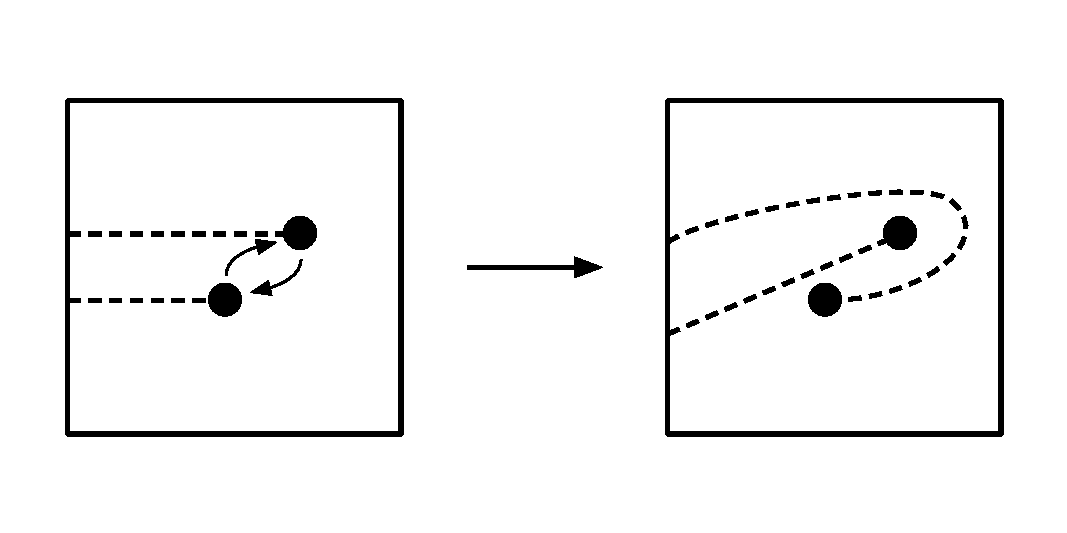
\includegraphics[width=0.5\textwidth]{./figures/pwave-braid.pdf}
  \caption{Two vortices in an elementary braid exchange.}
  \label{fig:pwave-braid}
\end{figure}


This change of sign is important in braiding transformations since it allows for non-Abelian exchange statistics.
We can circumvent a global phase by introducing branch cuts for the vortices to cross, causing a $2\pi$ phase change in the MFs.
Vortices can be exchanged as described in Figure ~\ref{fig:pwave-braid}, with a "bird's eye" view.
We can define the braiding operators as the following

\begin{equation}
  T_i :
  \begin{cases}
    \gamma_i \mapsto \gamma_{i+1} \\
    \gamma_{i+1} \mapsto -\gamma_i \\
    \gamma_j \mapsto \gamma_j \quad\quad \text{for $j\neq i$ and $j\neq i+1$}.
  \end{cases}
\end{equation}
This leads to the following braiding relations

\begin{figure}
  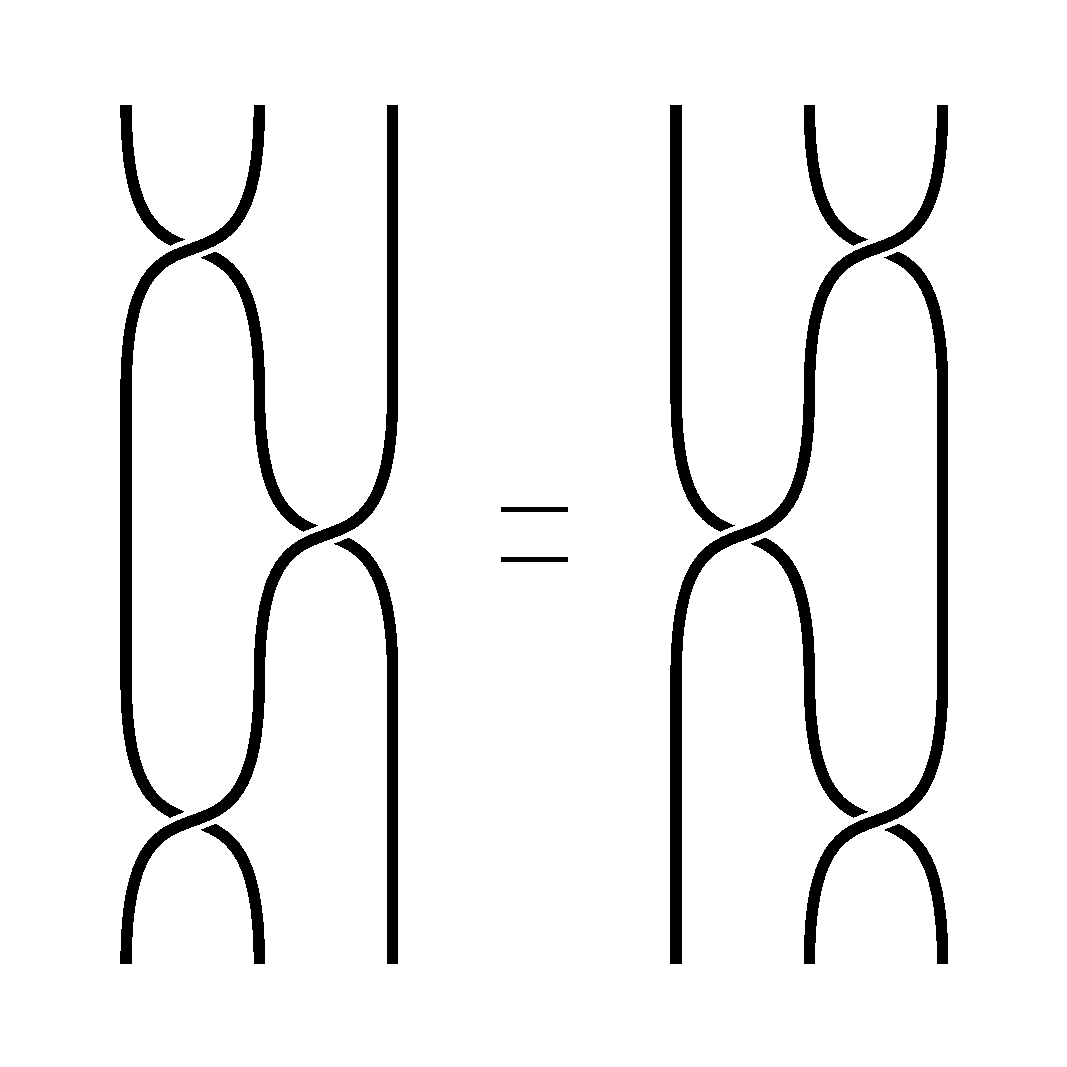
\includegraphics[width=0.33\textwidth]{./figures/braid.pdf}
  \caption{Braid group relation for $T_i T_{i+1} T_i = T_{i+1} T_i T_{i+1}$.}
  \label{fig:braid}
\end{figure}
\begin{equation}
  \begin{align*}
    T_i T_j = T_j T_i, \quad |i-j| > 1, \\
    T_i T_j T_i = T_j T_i T_j, \quad |i-j| = 1.
  \end{align*}
\end{equation}
Figure ~\ref{fig:braid} demonstrates three neighboring vortices with braiding statistics having two means of achieving the same braiding exchange.
One can write the braiding operators in terms of fermionic operators with the following

\begin{equation}
  \tau(T_i) = \exp\left(\dfrac{\pi}{4} \gamma_{i+1} \gamma_i\right) = \dfrac{1}{\sqrt{2}} \left(1+ \gamma_{i+1} \gamma_i\right).
\end{equation}
This can be further carried out for any number of MFs and builds a set of braiding operators for that system.

\begin{figure}[t]
  \begin{tikzpicture}
    \node[inner sep=0pt] (f1) at (-3,0) {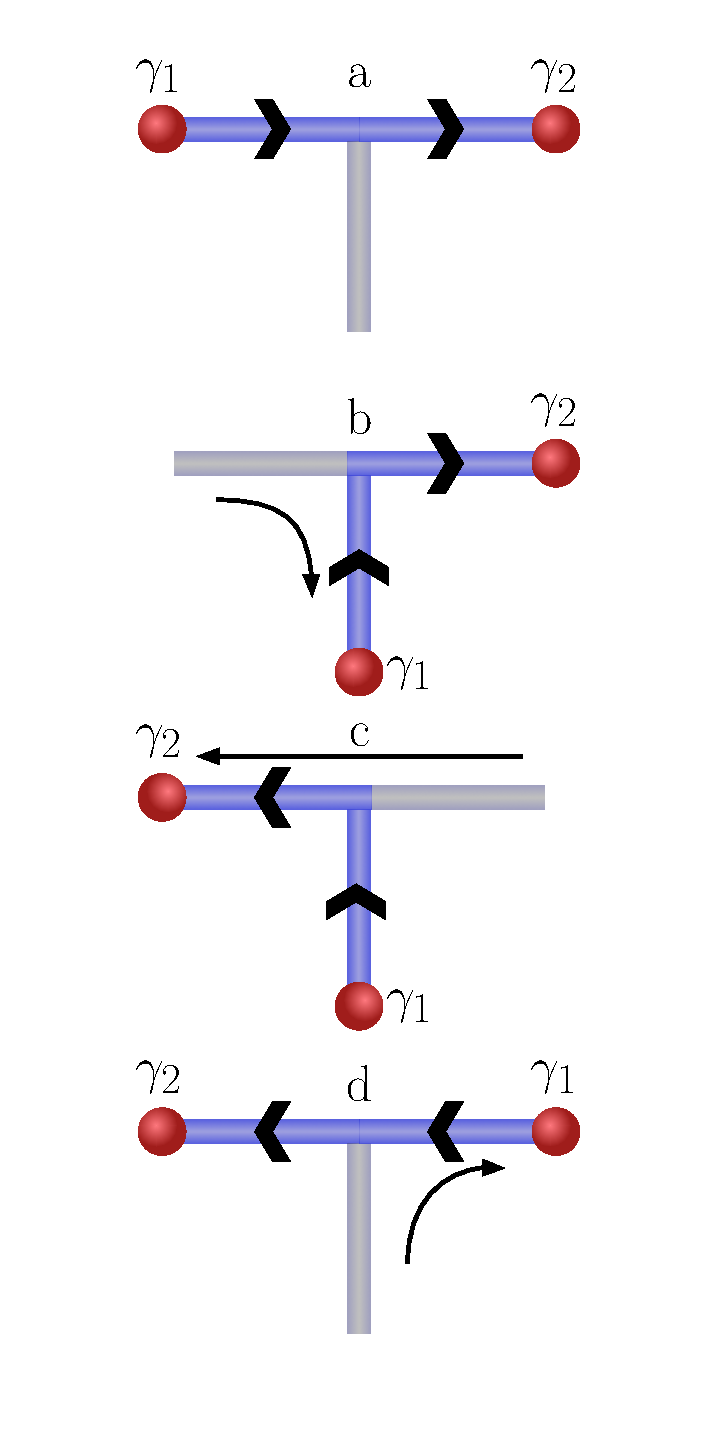
\includegraphics[width=0.25\textwidth]{./figures/t-junction-braid.pdf}};
    \node[inner sep=0pt] (f2) at (3,0) {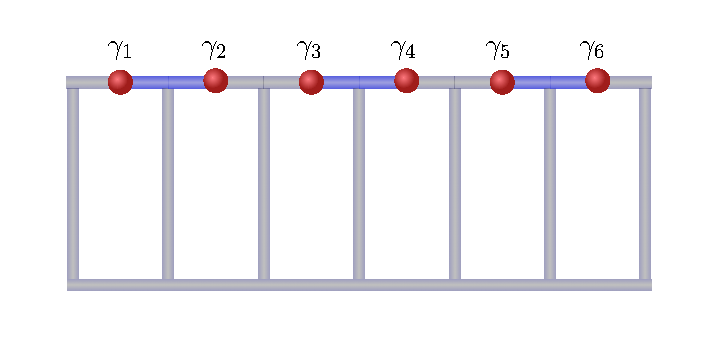
\includegraphics[width=0.5\textwidth]{./figures/ladder-junction.pdf}};
  \end{tikzpicture}
  \caption{(Left) Braiding two MFs on a T-junction. (Right) Ladder junction schematic for hosting and braiding multiple MFs.}
  \label{fig:t-junction-braid}
\end{figure}

\subsection{T-junction qubit}
The simplest qubit theorized for braiding MFs is on 1D wires connected in a T-junction, which can be extrapolated to a ladder junction for $2n$ MFs.
In the T-junction we define the quasi-1D Hamiltonian

\begin{equation}
  \ham = -\mu \sum_j \cc_j c_j - \sum_j \left(t\cc_j c_{j+1} + |\Delta|e^{i\phi} c_j c_{j+1} + h.c. \right),
\end{equation}
where
$c_j = e^{-i\phi/2} (\gamma_{j+1,1} + i \gamma_{j,2})/2$.
We additionally have to define the pairing as
$|\Delta|e^{i\phi} c_j c_{j+1}$
such that the site indices have the following definitions
\begin{itemize}
  \item Increase moving $\rightarrow / \uparrow$ in the horizontal/vertical wires: $\phi = 0$,
  \item Decrease moving $\leftarrow / \downarrow$ in the horizontal/vertical wires: $\phi = \pi$.
\end{itemize}
The braiding of two MFs in a T-junction is achieved by adiabatically tuning the voltage gate, or chemical potential, of the wires which can be seen in Figure ~\ref{fig:t-junction-braid}.
The process can be extrapolated to a ladder junction as shown in Figure ~\ref{fig:t-junction-braid} ~\cite{aliceaNonAbelianStatisticsTopological2011}.
While this approach is simple in theory and being seriously pursued, it is difficult to build, manipulate, and read experimentally.
Another difficulty for these wires is that there are no pristine \textit{p}-wave superconductors known to date, while effective \textit{p}-wave superconductors made of heterostructures, to be introduced next, are prone to various artifacts.

